% Options for packages loaded elsewhere
\PassOptionsToPackage{unicode}{hyperref}
\PassOptionsToPackage{hyphens}{url}
%
\documentclass[
  ,jou,floatsintext]{apa6}
\usepackage{amsmath,amssymb}
\usepackage{lmodern}
\usepackage{iftex}
\ifPDFTeX
  \usepackage[T1]{fontenc}
  \usepackage[utf8]{inputenc}
  \usepackage{textcomp} % provide euro and other symbols
\else % if luatex or xetex
  \usepackage{unicode-math}
  \defaultfontfeatures{Scale=MatchLowercase}
  \defaultfontfeatures[\rmfamily]{Ligatures=TeX,Scale=1}
\fi
% Use upquote if available, for straight quotes in verbatim environments
\IfFileExists{upquote.sty}{\usepackage{upquote}}{}
\IfFileExists{microtype.sty}{% use microtype if available
  \usepackage[]{microtype}
  \UseMicrotypeSet[protrusion]{basicmath} % disable protrusion for tt fonts
}{}
\makeatletter
\@ifundefined{KOMAClassName}{% if non-KOMA class
  \IfFileExists{parskip.sty}{%
    \usepackage{parskip}
  }{% else
    \setlength{\parindent}{0pt}
    \setlength{\parskip}{6pt plus 2pt minus 1pt}}
}{% if KOMA class
  \KOMAoptions{parskip=half}}
\makeatother
\usepackage{xcolor}
\usepackage{graphicx}
\makeatletter
\def\maxwidth{\ifdim\Gin@nat@width>\linewidth\linewidth\else\Gin@nat@width\fi}
\def\maxheight{\ifdim\Gin@nat@height>\textheight\textheight\else\Gin@nat@height\fi}
\makeatother
% Scale images if necessary, so that they will not overflow the page
% margins by default, and it is still possible to overwrite the defaults
% using explicit options in \includegraphics[width, height, ...]{}
\setkeys{Gin}{width=\maxwidth,height=\maxheight,keepaspectratio}
% Set default figure placement to htbp
\makeatletter
\def\fps@figure{htbp}
\makeatother
\setlength{\emergencystretch}{3em} % prevent overfull lines
\providecommand{\tightlist}{%
  \setlength{\itemsep}{0pt}\setlength{\parskip}{0pt}}
\setcounter{secnumdepth}{-\maxdimen} % remove section numbering
% Make \paragraph and \subparagraph free-standing
\ifx\paragraph\undefined\else
  \let\oldparagraph\paragraph
  \renewcommand{\paragraph}[1]{\oldparagraph{#1}\mbox{}}
\fi
\ifx\subparagraph\undefined\else
  \let\oldsubparagraph\subparagraph
  \renewcommand{\subparagraph}[1]{\oldsubparagraph{#1}\mbox{}}
\fi
\newlength{\cslhangindent}
\setlength{\cslhangindent}{1.5em}
\newlength{\csllabelwidth}
\setlength{\csllabelwidth}{3em}
\newlength{\cslentryspacingunit} % times entry-spacing
\setlength{\cslentryspacingunit}{\parskip}
\newenvironment{CSLReferences}[2] % #1 hanging-ident, #2 entry spacing
 {% don't indent paragraphs
  \setlength{\parindent}{0pt}
  % turn on hanging indent if param 1 is 1
  \ifodd #1
  \let\oldpar\par
  \def\par{\hangindent=\cslhangindent\oldpar}
  \fi
  % set entry spacing
  \setlength{\parskip}{#2\cslentryspacingunit}
 }%
 {}
\usepackage{calc}
\newcommand{\CSLBlock}[1]{#1\hfill\break}
\newcommand{\CSLLeftMargin}[1]{\parbox[t]{\csllabelwidth}{#1}}
\newcommand{\CSLRightInline}[1]{\parbox[t]{\linewidth - \csllabelwidth}{#1}\break}
\newcommand{\CSLIndent}[1]{\hspace{\cslhangindent}#1}
\ifLuaTeX
\usepackage[bidi=basic]{babel}
\else
\usepackage[bidi=default]{babel}
\fi
\babelprovide[main,import]{english}
% get rid of language-specific shorthands (see #6817):
\let\LanguageShortHands\languageshorthands
\def\languageshorthands#1{}
% Manuscript styling
\usepackage{upgreek}
\captionsetup{font=singlespacing,justification=justified}

% Table formatting
\usepackage{longtable}
\usepackage{lscape}
% \usepackage[counterclockwise]{rotating}   % Landscape page setup for large tables
\usepackage{multirow}		% Table styling
\usepackage{tabularx}		% Control Column width
\usepackage[flushleft]{threeparttable}	% Allows for three part tables with a specified notes section
\usepackage{threeparttablex}            % Lets threeparttable work with longtable

% Create new environments so endfloat can handle them
% \newenvironment{ltable}
%   {\begin{landscape}\centering\begin{threeparttable}}
%   {\end{threeparttable}\end{landscape}}
\newenvironment{lltable}{\begin{landscape}\centering\begin{ThreePartTable}}{\end{ThreePartTable}\end{landscape}}

% Enables adjusting longtable caption width to table width
% Solution found at http://golatex.de/longtable-mit-caption-so-breit-wie-die-tabelle-t15767.html
\makeatletter
\newcommand\LastLTentrywidth{1em}
\newlength\longtablewidth
\setlength{\longtablewidth}{1in}
\newcommand{\getlongtablewidth}{\begingroup \ifcsname LT@\roman{LT@tables}\endcsname \global\longtablewidth=0pt \renewcommand{\LT@entry}[2]{\global\advance\longtablewidth by ##2\relax\gdef\LastLTentrywidth{##2}}\@nameuse{LT@\roman{LT@tables}} \fi \endgroup}

% \setlength{\parindent}{0.5in}
% \setlength{\parskip}{0pt plus 0pt minus 0pt}

% Overwrite redefinition of paragraph and subparagraph by the default LaTeX template
% See https://github.com/crsh/papaja/issues/292
\makeatletter
\renewcommand{\paragraph}{\@startsection{paragraph}{4}{\parindent}%
  {0\baselineskip \@plus 0.2ex \@minus 0.2ex}%
  {-1em}%
  {\normalfont\normalsize\bfseries\itshape\typesectitle}}

\renewcommand{\subparagraph}[1]{\@startsection{subparagraph}{5}{1em}%
  {0\baselineskip \@plus 0.2ex \@minus 0.2ex}%
  {-\z@\relax}%
  {\normalfont\normalsize\itshape\hspace{\parindent}{#1}\textit{\addperi}}{\relax}}
\makeatother

% \usepackage{etoolbox}
\makeatletter
\patchcmd{\HyOrg@maketitle}
  {\section{\normalfont\normalsize\abstractname}}
  {\section*{\normalfont\normalsize\abstractname}}
  {}{\typeout{Failed to patch abstract.}}
\patchcmd{\HyOrg@maketitle}
  {\section{\protect\normalfont{\@title}}}
  {\section*{\protect\normalfont{\@title}}}
  {}{\typeout{Failed to patch title.}}
\makeatother

\usepackage{xpatch}
\makeatletter
\xapptocmd\appendix
  {\xapptocmd\section
    {\addcontentsline{toc}{section}{\appendixname\ifoneappendix\else~\theappendix\fi\\: #1}}
    {}{\InnerPatchFailed}%
  }
{}{\PatchFailed}
\usepackage{dblfloatfix}


\usepackage{csquotes}
\ifLuaTeX
  \usepackage{selnolig}  % disable illegal ligatures
\fi
\IfFileExists{bookmark.sty}{\usepackage{bookmark}}{\usepackage{hyperref}}
\IfFileExists{xurl.sty}{\usepackage{xurl}}{} % add URL line breaks if available
\urlstyle{same} % disable monospaced font for URLs
\hypersetup{
  pdftitle={Faith in Reason: developing a survey measure of belief in the rationality of others},
  pdfauthor={Tom Stafford1, Junyan Zhu2, \& Katharine Dommett2},
  pdflang={en-EN},
  hidelinks,
  pdfcreator={LaTeX via pandoc}}

\title{Faith in Reason: developing a survey measure of belief in the rationality of others}
\author{Tom Stafford\textsuperscript{1}, Junyan Zhu\textsuperscript{2}, \& Katharine Dommett\textsuperscript{2}}
\date{}


\shorttitle{Faith in Reason}

\authornote{

For the purpose of open access, the author has applied a Creative Commons Attribution (CC BY) licence to any Author Accepted Manuscript version arising.

Document prepared with RMarkdown (Allaire et al., 2020) and papaja (Aust \& Barth, 2020). CRediT (Contributor Roles Taxonomy) autogenerated using Tenzing (Holcombe, Kovacs, Aust, \& Aczel, 2020). Template is available here \href{https://github.com/tomstafford/rmarkdown_apa}{github.com/tomstafford/rmarkdown\_apa}

The authors made the following contributions. Tom Stafford: Conceptualization, Data curation, Formal analysis, Funding acquisition, Methodology, Visualization, Writing - original draft, Writing - review \& editing; Junyan Zhu: Conceptualization, Data curation, Formal analysis, Methodology, Writing - review \& editing; Katharine Dommett: Conceptualization, Funding acquisition, Methodology, Writing - review \& editing.

Correspondence concerning this article should be addressed to Tom Stafford, Department of Psychology, University of Sheffield, Sheffield, UK. E-mail: \href{mailto:t.stafford@sheffield.ac.uk}{\nolinkurl{t.stafford@sheffield.ac.uk}}

}

\affiliation{\vspace{0.5cm}\textsuperscript{1} Department of Psychology, University of Sheffield, UK\\\textsuperscript{2} Department of Politics and International Relations, University of Sheffield, UK}

\note{\textcolor{red}{Draft 2023-04-28}}

\abstract{%
What we believe about other people matters. It is not enough that others \emph{are} trustworthy, reasonable or well intentioned. Successful coordination, as well as individual wellbeing, benefit when we also \emph{perceive} others as trustworthy, reasonable or well intentioned. While standard measures of trust and benevolence exist, there is no standard measure of the generalised belief in the rationality or reasonableness of other people. Here, we present the development and testing of a scale to directly measure this attitude. Using a representative sample of 1869 UK adults, we test dimensionality and consistency of the scale items. We show that the refined, six-item, scale is associated with, but not entirely determined by, generalised trust in other people. Our ``Faith in Reason'' scale shows large individual differences, but the average tendency is slightly on the side of endorsing, rather than rejecting, sentiments such as ``The typical person is often irrational''.
}



\begin{document}
\maketitle

\hypertarget{introduction}{%
\section{Introduction}\label{introduction}}

\hypertarget{rationality}{%
\subsection{Rationality}\label{rationality}}

\begin{quote}
\emph{All our dignity consists then in thought. By it we must elevate ourselves, and not by space and time which we cannot fill. Let us endeavour then to think well; this is the principle of morality.}
Pascal (1669/1910)
\end{quote}

The nature of human reason is a perennial topic. Human rationality has often been praised (``Man is but a reed, the most feeble thing in nature, but he is a thinking reed,'' Pascal, 1669/1910), but so have its failures condemned been by many different thinkers.

An influential account of human reasoning is provided by the heuristics and biases programme (Kahneman, Slovic, \& Tversky, 1982), which uses the ideal of economic rationality as a standard to define actual human reasoning against. From this perspective human reasoning appears riddled with biases, but much of this effect is due to the adoption of the standards of utility theory, formal logic and precise statistical reasoning against which to define error. Critics have questions the appropriateness of these standards (e.g. Gigerenzer \& Gaissmaier, 2011). The logic of controlled experiments allows researchers to isolate and emphasise quirks in human reasoning, while backgrounding reason-responsiveness (Stafford, 2014). Accordingly, the psychology literature may overemphasise the role of error, bias and motivated reasoning (Stafford, 2020). The debate has been so heated in the cognitive sciences that `Rationality Wars' (Samuels, Stich, \& Bishop, 2002) have been declared over the definition of rationality that might reasonably used as a standard against which to judge human reasoning.

Mercier and Sperber's (2011) Argumentative Theory of Reason provides an interactionist, rather than individualist account of human reasoning, which emphasises the social context in which human reasoning evolved. This account suggests, among other things, the importance of dialogue based argumentation in changing beliefs (Brand \& Stafford, 2022; Karadzhov, Stafford, \& Vlachos, 2022) and the validity of incorporating social factors like the status, trustworthiness or expertise of a source of information in the reasoning process (Eiser, Stafford, Henneberry, \& Catney, 2009).

\hypertarget{criteria-of-reason}{%
\subsection{Criteria of reason}\label{criteria-of-reason}}

So rationality is not a unitary concept, nor one around which there is consensus on the definition of, despite the way it is often evoked in discussion (and particularly in discussion of its negation e.g.~``they are being irrational''). That said, core features of rationality have been proposed, and it may be possible to test these as aspects of the `folk theory' of rationality that exists in the common understanding.

Two primary criteria are `\textbf{correspondence}', where beliefs are aligned with reality (in the form of the state of the world or their behaviour), and `\textbf{coherence}', where beliefs are aligned with each other (i.e.~consistent, but see Sommer, Musolino, and Hemmer (2022)). For more on corresponence and coherance see Dawson and Gregory (2009).

Another criteria of rationalty which can be identified is \textbf{insight} into your own beliefs and how they guide behaviour. The rhetorical power of certain celebrated demonstrations of irrationality (e.g. Nisbett \& Wilson, 1977) relies on the surprise that people can act, supposedly, unaware of the causes of their behaviour (but see Stafford, 2020).

Finally, susceptibility to \textbf{influence} is a key aspect of rationality (Mercier, 2020). This can be positively construed - to be rational is to be responsive to reasons, persuadable by evidence and so on. And it can be negative construed - to be irrational is to be gullible, or stubborn in the face of good reasons to change your mind.

So core features of rationality include coherence, correspondence, susceptibility to influence and insight into causes of ones actions. The extent to which these features form a coherent whole in the minds of the general public, and can meaningfully be asked about questions about is a primary question of this paper.

\hypertarget{consequence-of-a-lack-of-faith-in-reason}{%
\subsection{Consequence of a lack of faith in reason}\label{consequence-of-a-lack-of-faith-in-reason}}

Investigating folk conceptions of rationality is not just interesting in its own right, individual's beliefs about the rationality of others may be important for a number of other core beliefs and behaviours.

\hypertarget{second-order-effects-of-disinformation}{%
\subsubsection{Second order effects of disinformation}\label{second-order-effects-of-disinformation}}

The generalised belief that others are well informed and reasonable is foundational to democracy. Recent concerns around misinformation may have second order effects, undermining democracy not by generating a misinformed populace, but by generating a populace that believes others are misunformed or unreasonable (Karpf, 2019). Alarmism around misinformation may potentially lower trust in institutions (Hoes, Clemm von Hohenberg, Gessler, Wojcieszak, \& Qian, 2022), increase skepticism about democracy (Jungherr \& Rauchfleisch, 2022; Nisbet, Mortenson, \& Li, 2021), or foster calls of tighter media regulation (Lee, 2021). Altay and Acerbi (2023) have shown that the threat of misinformation is directly related to the perceptions of others' gullibility.

\hypertarget{third-person-effect}{%
\subsubsection{Third person effect}\label{third-person-effect}}

There is an established literature of the perception of media influence on others (Perloff, 2002; Sun, Pan, \& Shen, 2008). The `third person effect', proposed by Davison (1983), is the phenomenon whereby many people believe others are more susceptible to influence than themselves. The third person effect was proposed as a root cause of censorship instincts and this has been confirmed by subsequent empricial investigations (Feng \& Guo, 2012; Olshansky \& Landrum, 2020).

Two caveats around the third person effect. Lyons (2022) has recently argued that - for many people - a third person effect of greater media influence on others rather than the self will be an accurate perception. Chung and Moon (2016) have argued that the driving factor in many so-called third person effects is the perception of others (as highly influenced), rather than the discrepancy with first person perception per se.

\hypertarget{generalised-trust-value-of-democracy}{%
\subsection{Generalised trust \& value of democracy}\label{generalised-trust-value-of-democracy}}

Generalised trust is the belief that, `most people can be trusted' (Brehm \& Rahn, 1997; Paxton, 1999). It is reflected in standard items in long running time series surveys such as the World Values Survey (Inglehart \& Team, 2023) an the General Social Survey (General Social Survey Team, 2023). Generalised trust is an aspect of social capital, broadly conceived (Putnam, 2000) and as such as an important aspect of wellbeing and the health of society (Cohn, Maréchal, Tannenbaum, \& Zünd, 2019). Given the recognised importance of generalised trust, it is nature to ask how other beliefs feed into this belief. Why do we trust others? Do we trust them intellectually as well as morally? Do we think other people are able to work things out for themselves, to display good judgement? Do we trust the typical person to avoid being manipulated, to respond to arguments, to reason their way to good enough decisions? In short, is generalised trust informed by beliefs about the rationality or reasonableness of others?

Similarly, attitudes to demoracy may mutually inform beliefs about the reasonableness of one's fellow citizens. One standardised measure of attitude to democracy is the item from the World Values Survey (Inglehart \& Team, 2023) which asks `How important is it for you to live in a country that is governed democratically?'.

\hypertarget{lack-of-existing-measures}{%
\subsection{Lack of existing measures}\label{lack-of-existing-measures}}

To our knowledge, no existing scale directly measures belief in reasoning. There are scales which measure related concepts, or concepts which are plausible antecedents or consequences of belief in the reasonableness of our fellow citizens. In addition to the measures of generalised trust discussed above, there are also measures of conspiracy beliefs or mentality (see Swami et al., 2017 for a brief review) including those which explicitly try to distinguish conspiracist from rational skepticism (Stojanov, Bering, \& Halberstadt, 2020; Stojanov \& Halberstadt, 2019). These do not direct assess rationality, and again could be viewed a more alike to measuring a consequence of rationality or a lack of it (i.e.~due to manipulation or credulity).

Some researchers have looked at what they call `cynical beliefs about human nature' (e.g. Stavrova \& Ehlebracht, 2016), but these, again, do not touch on reason or rationality as a cause of cynicism. Instead, scale items are similar to generalised trust/distrust measures.

Other studies have looked at beliefs about human nature (e.g. Furnham, Johnson, \& Rawles, 1985). These have questions which focus on the role of biology, genetics and/or heredity on psychological traits. For example, asking if participants believe personality is entirely caused by a person's genetics. Again, these scales do not directly assess beliefs about human reason, although they do assess beliefs which may plausibly affect beliefs about human reason.

\hypertarget{summary}{%
\subsection{Summary}\label{summary}}

In summary, generalised belief in the rationality or reasonableness of others is interesting in its own right, in relation to longstanding debates in the cognitive sciences about the definition of rationality and due to plausible relation to other atittudes recognised of importance, such as generalised trust. To our knowledge, no scale exists which directly measures this generalised belief. To develop, refine and explore such a scale is the purpose of the current study.

\hypertarget{method}{%
\section{Method}\label{method}}

\hypertarget{sample}{%
\subsection{Sample}\label{sample}}

The questions were asked as part of a larger survey experiment (Zhu, Dommett, \& Stafford, submitted), in which participants were asked to view adverts which appeared on Facebook during the 2019 UK general election. Participants were recruited via the online platform Prolific. In terms of age, gender, regional dispersion and political affiliations participants reflected a representative sample of UK adults. Data was collected on 2022-08-20. Full details are give in Zhu et al. (submitted).

\hypertarget{item-development}{%
\subsection{Item development}\label{item-development}}

In order to develop the scale items, we developed eight items, informed by the debates in cognitive science around the nature of rationality (see introduction). Half of these were positively framed, to reflect endorsement of human's tendency towards rationality and reasonableness. Half were negatively framed, to reflect endorsement of a tendency towards irrationality and unreasonableness. Items, their framing (positive/negative) and the aspect of rationality they were designed to capture are shown in Table \ref{tab:items}.

\begin{table*}[tbp]

\begin{center}
\begin{threeparttable}

\caption{\label{tab:items}Scale item wording}

\begin{tabular}{llll}
\toprule
Item & \multicolumn{1}{c}{Framing} & \multicolumn{1}{c}{Aspect} & \multicolumn{1}{c}{Wording}\\
\midrule
1 & negative & general & The typical person is often irrational\\
2 & negative & corresponence & People are often misinformed on important issues\\
3 & negative & influence & People are too easily manipulated\\
4 & negative & insight & People often act for reasons they don’t understand or endorse\\
5 & positive & influence & The average person can be persuaded to change their mind if given good reasons\\
6 & positive & correspondence & Most people hold accurate views about the world\\
A & NA & ATTN CHECK & For this question please click the middle option, ‘neutral’, to show you are paying attention\\
7 & positive & coherance & An individual's beliefs about the world are generally coherent\\
8 & positive & coherance & People's behaviour is generally consistent with their beliefs\\
\bottomrule
\addlinespace
\end{tabular}

\begin{tablenotes}[para]
\normalsize{\textit{Note.} Response was on a 7 point Likert scale from (1 = "Strongly Disagree", 7 = "Strongly Agree"). Items 1,2,3 and 4 reverse coded so that for all items higher scores represented stronger faith in reason.}
\end{tablenotes}

\end{threeparttable}
\end{center}

\end{table*}

In all analyses negatively framed items were reverse coded, so that numerically higher scores always reflect greater endorsement of human rationality, across all items. An attention check item was included in the scale (also shown in Table \ref{tab:items}).

\hypertarget{other-items}{%
\subsection{Other items}\label{other-items}}

Other items we report from the original survey are a measure of generalised trust (`Generally speaking, would you say that most people can be trusted?'), support for democracy (`How important is it for you to live in a country that is governed democratically?') and a measure of the Third Person Effect in the context of political advertising. This was calculated as the average response to six linked items about the influence of election advertising on the typical voter, with wording of the form specifically ``Thinking about the impact of political parties' election messages on the typical voter, to what extent do you agree or disagree that it helps to: - Raise their awareness of political issues; Raise their awareness of political candidates or parties; Prompt them to share messages related to the election; Prompt them to vote/ register to vote; Persuade them to change who you are planning to vote for; Influence how they feel about political opponents'. We also report demographic questions (age, sex, education)

\hypertarget{preregistration}{%
\subsection{Preregistration}\label{preregistration}}

Our analysis is supported by formal preregistration of hypothesis and data analyses practices
(OSF pre-registration link: \url{https://osf.io/y9kjg/?view_only=609cd46aab534e4c866c16b3ef29c510}). Note that the bulk of this preregistration concerns the analyses reported in Zhu et al. (submitted).

Preregistration supports the accurate identification of confirmatory versus exploratory analyses. The nature of scale development is necessarily exploratory, but the preregistration allows readers confirm what was intended and expected before data was collected.

\hypertarget{reproducibility}{%
\subsection{Reproducibility}\label{reproducibility}}

Data availability: The analysis code and anonymised response data which supports all results are openly available \url{https://github.com/tomstafford/faithinreason}

This repository contains the files used to generate this report, which is in the form of a `reproducible manuscript', a document which generates the analysis it reports, and so combines sharing, documenting and reporting an analysis in a single set of project files (Allaire et al., 2020 ; Aust \& Barth, 2020).

\hypertarget{results}{%
\section{Results}\label{results}}

\hypertarget{initial-characterisations}{%
\subsection{Initial characterisations}\label{initial-characterisations}}

Our data consist of 1875 participants who completed our online survey. 6 failed an attention check and were removed. Inital inspection suggested that a range of responses were obtain. For example, Figure \ref{fig:Q19item1} shows that the first item of the scale received the full range of responses from ``Strongly disagree'' to ``Strongly agree''.

\begin{figure}

{\centering 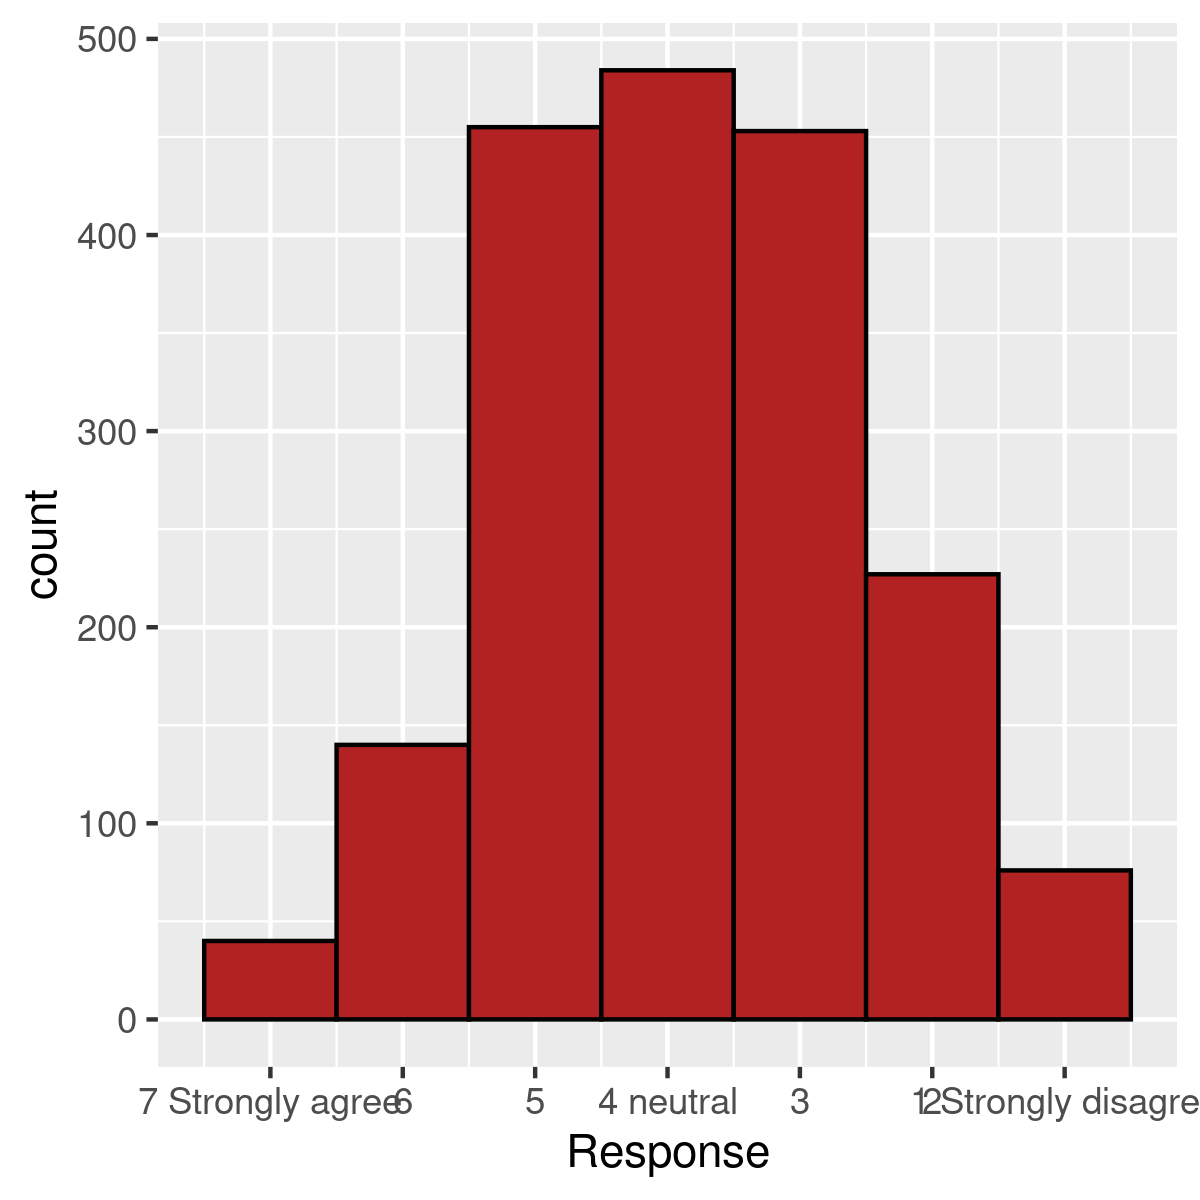
\includegraphics[width=0.75\linewidth]{faithinreason_files/figure-latex/Q19item1-1} 

}

\caption{Histogram of responses to Item 1 ("The typical person is often irrational")}\label{fig:Q19item1}
\end{figure}

\hypertarget{scale-development-assessing-dimensionality-item-selection}{%
\subsection{Scale development: assessing dimensionality \& item selection}\label{scale-development-assessing-dimensionality-item-selection}}

\begin{verbatim}
## Q19_1 
## 0.67 
## Q19_2 
## 0.67 
## Q19_3 
## 0.68 
## Q19_4 
## 0.68 
## Q19_5 
## 0.78 
## Q19_6 
## 0.67 
## Q19_8 
## 0.67 
## Q19_9 
## 0.7
\end{verbatim}

Cronbach's alpha is 0.72

\begin{figure}

{\centering 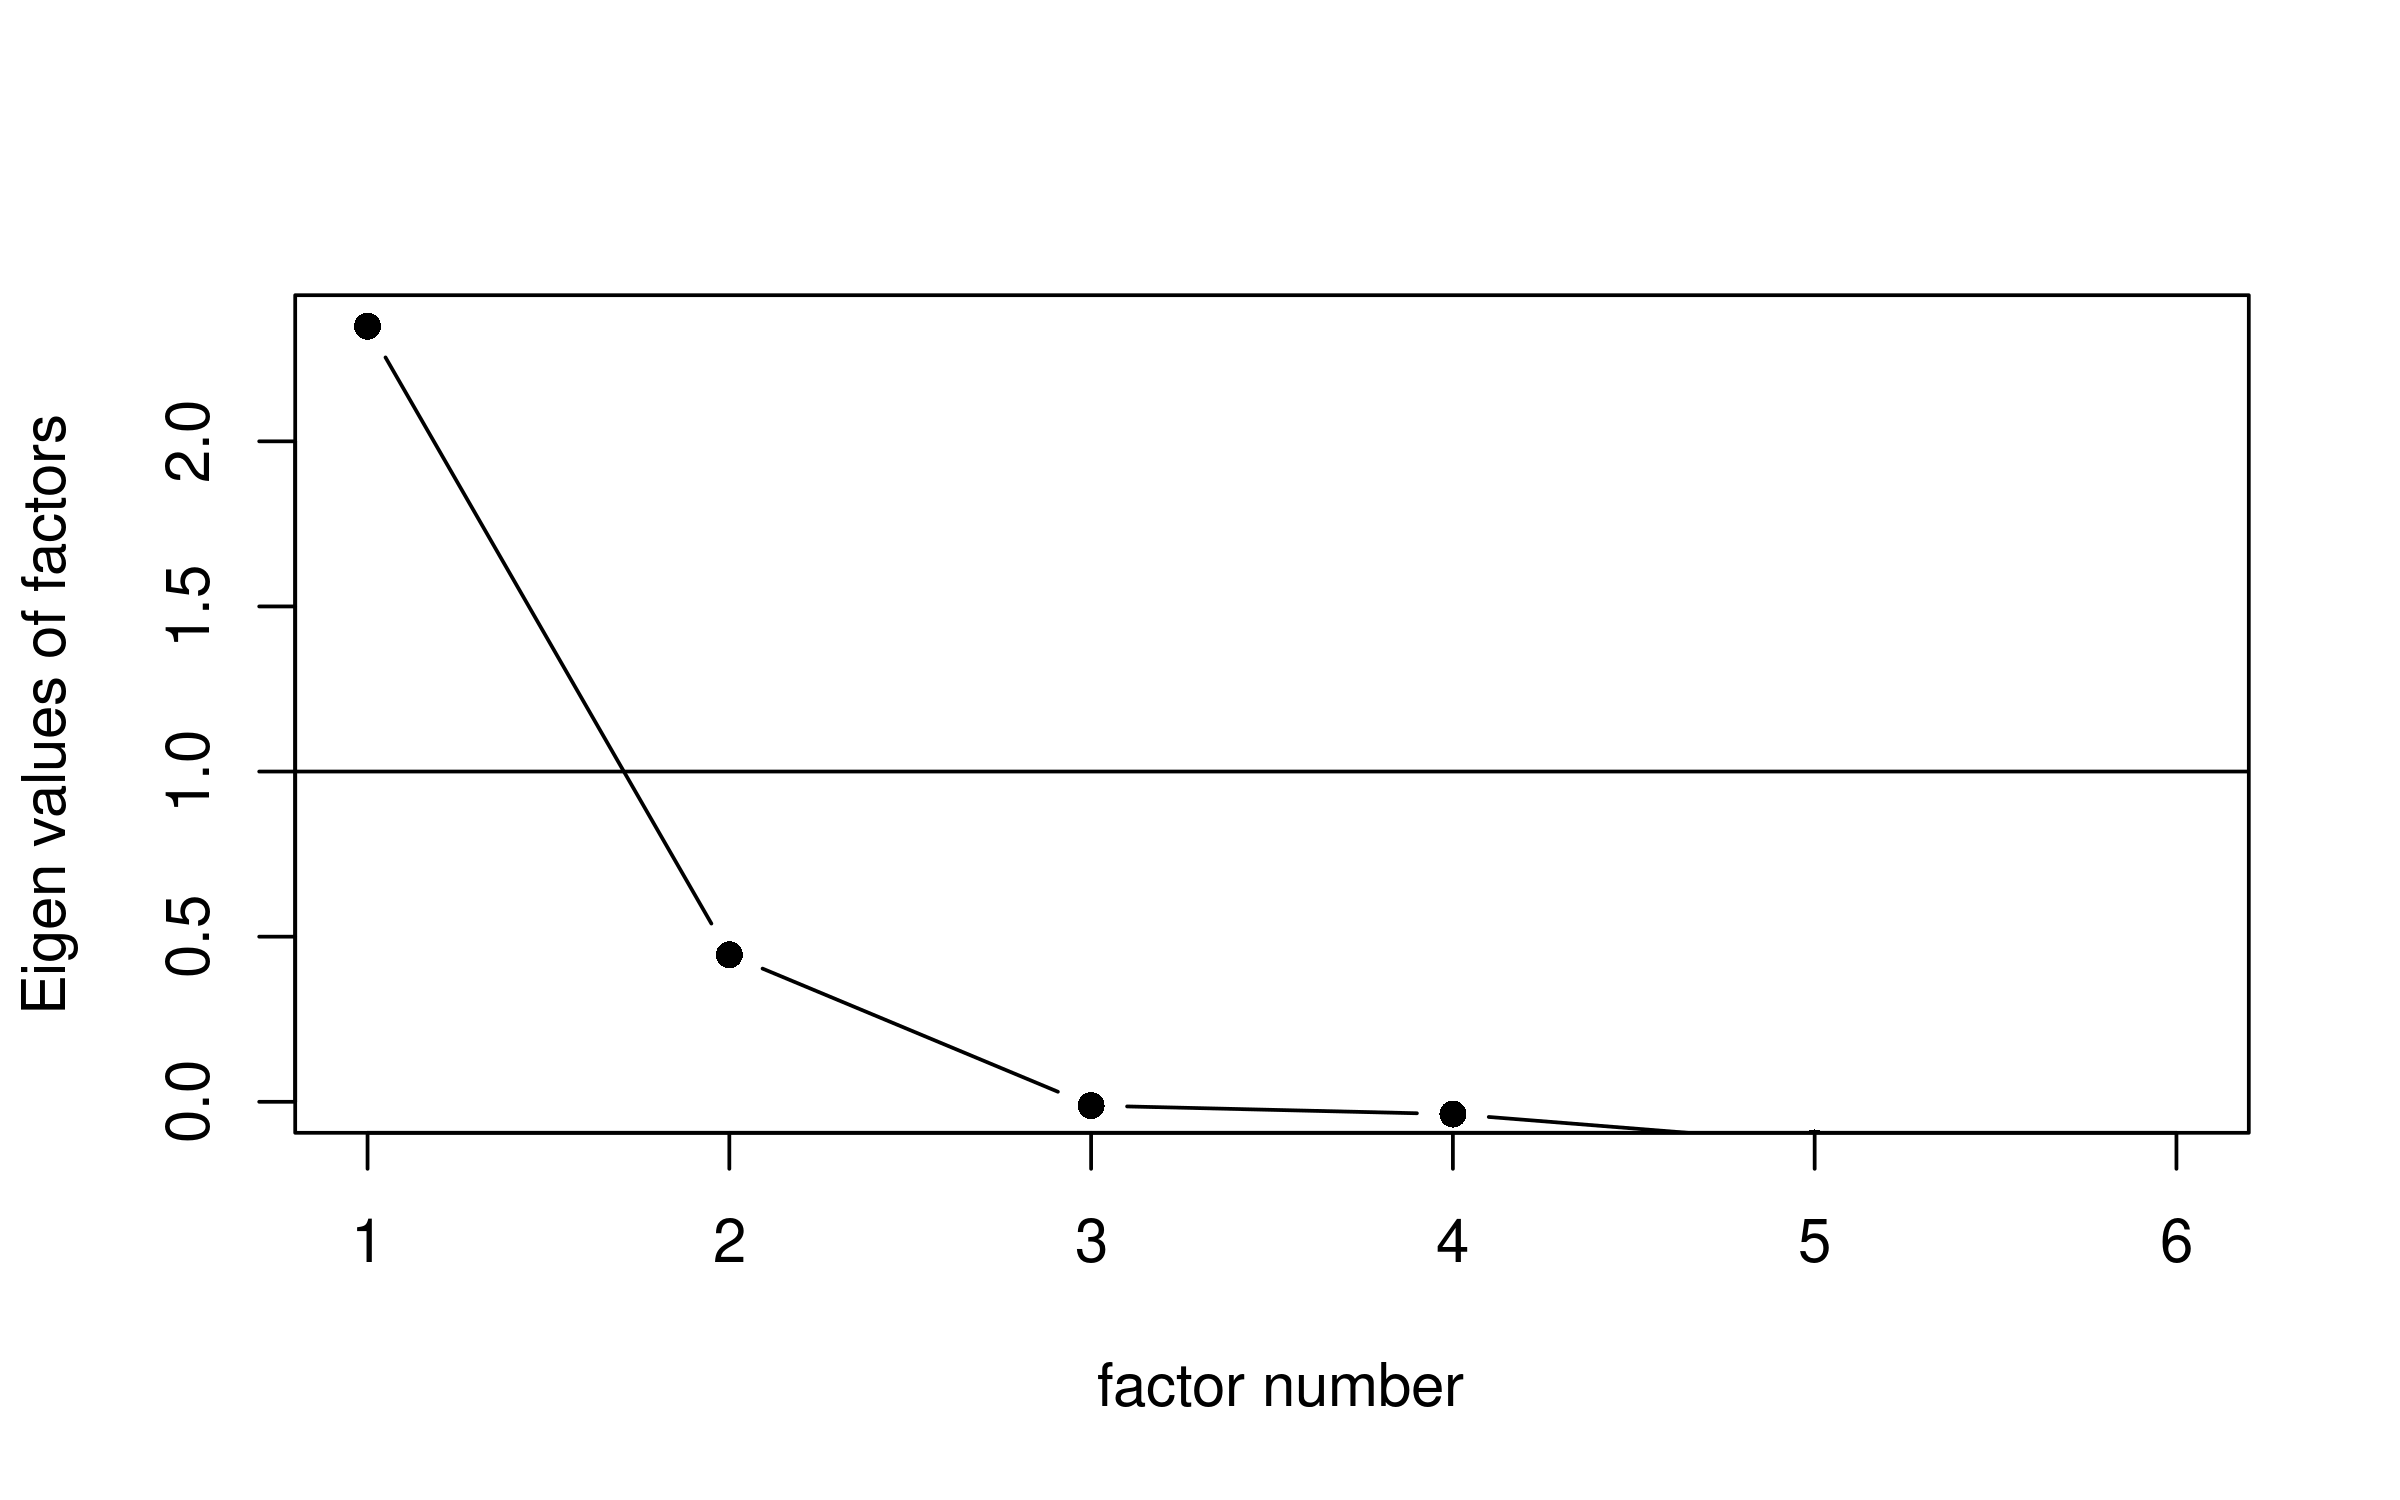
\includegraphics[width=1\linewidth]{plots/reason_scree6} 

}

\caption{Factor analysis}\label{fig:factors}
\end{figure}

\begin{figure}

{\centering 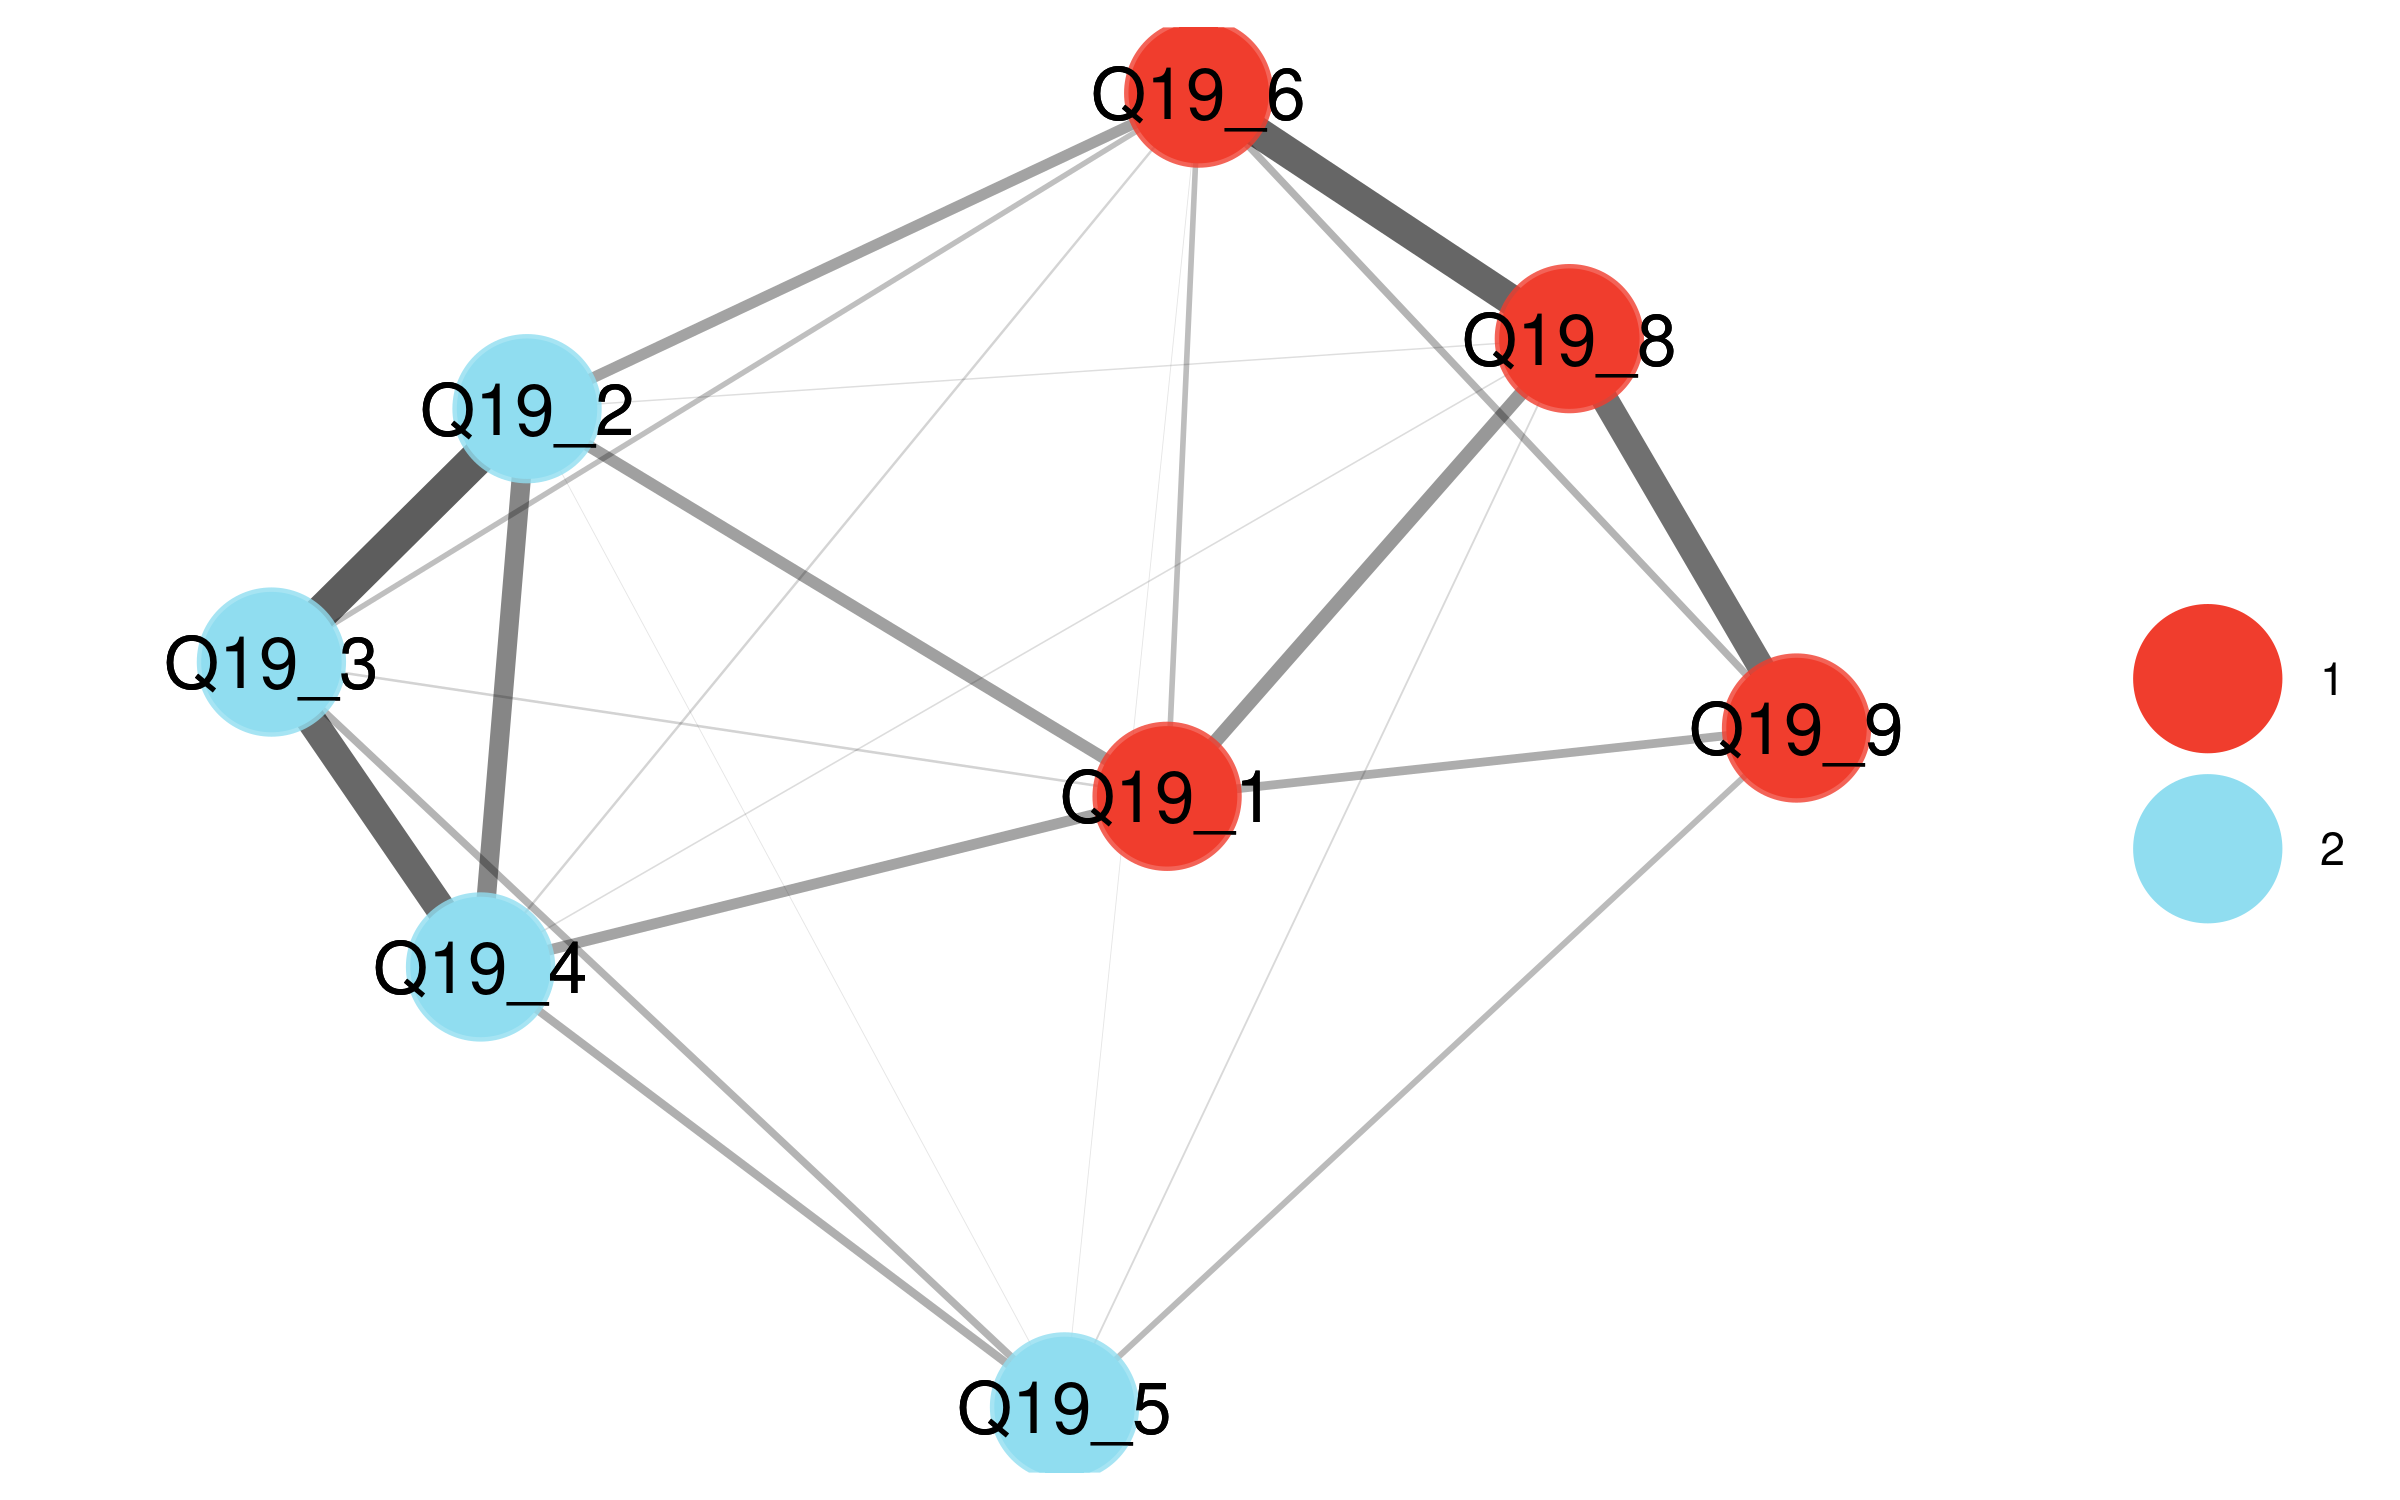
\includegraphics[width=1\linewidth]{plots/reason_ega} 

}

\caption{Exploratory Graph Analysis (EGA) of all items.}\label{fig:egafull}
\end{figure}

\begin{figure}

{\centering 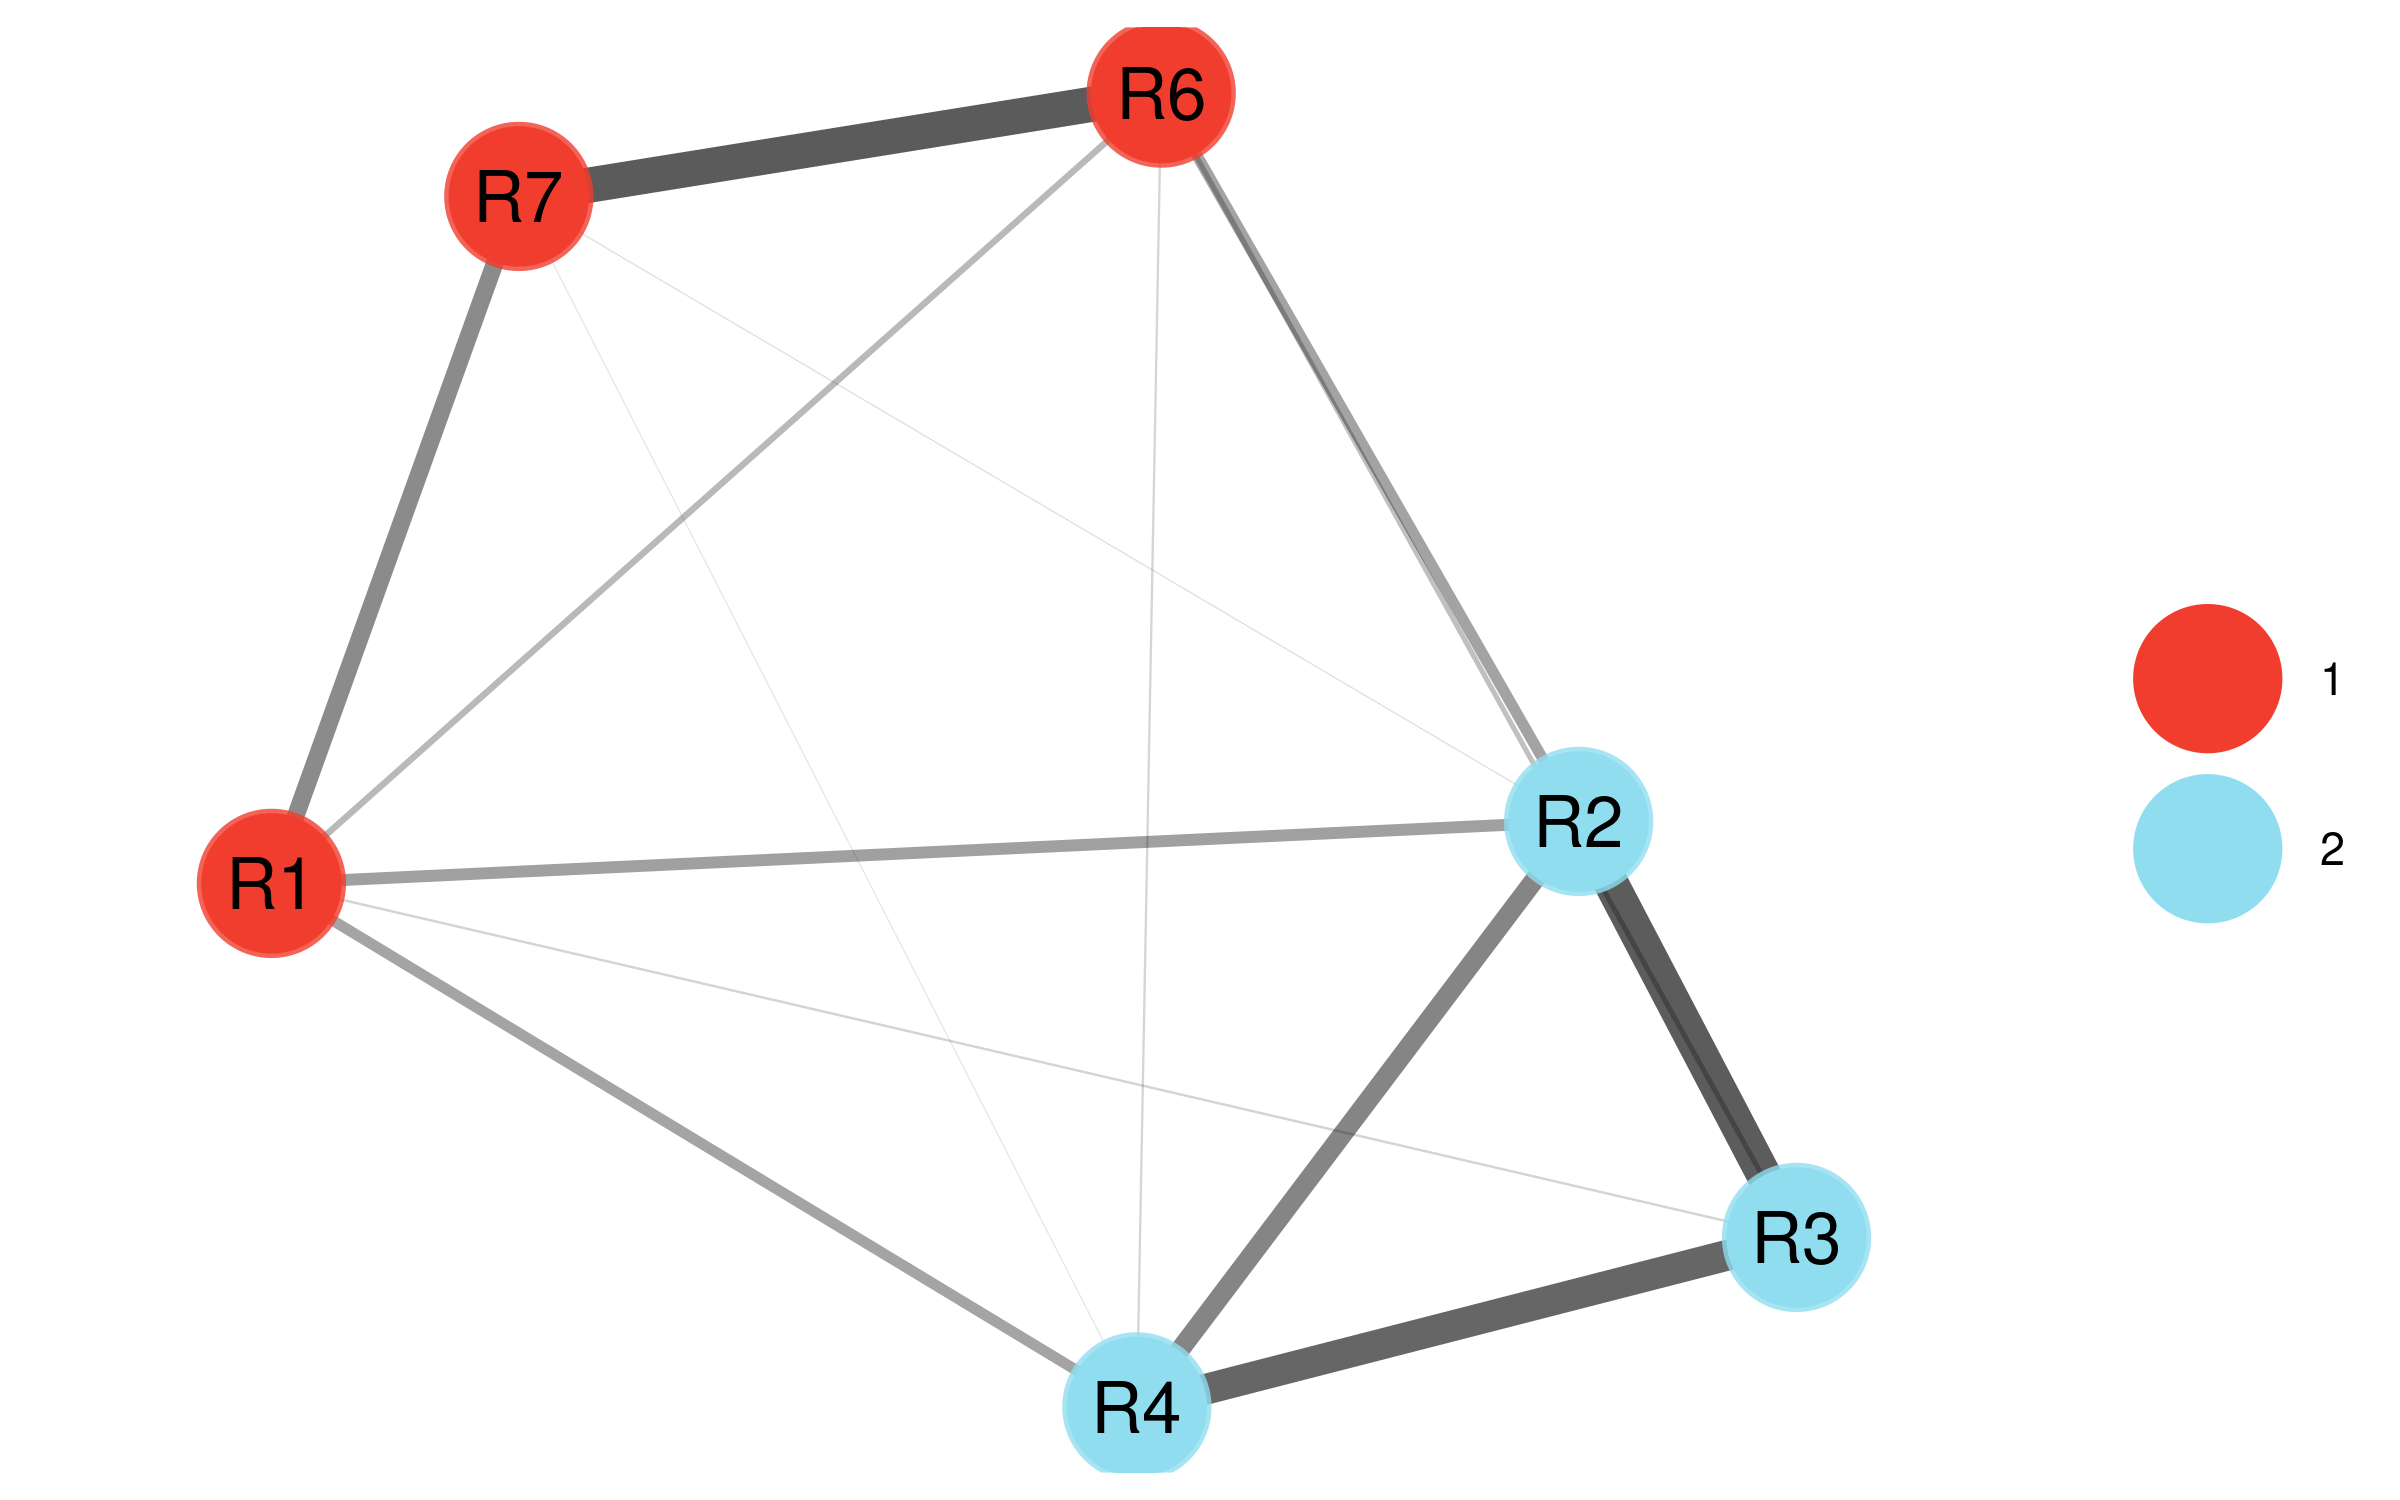
\includegraphics[width=1\linewidth]{plots/reason6_ega} 

}

\caption{The items of the full ASRS scale displayed following Exploratory Graph Analysis (EGA).}\label{fig:egasix}
\end{figure}

\hypertarget{scale-analysis}{%
\subsection{Scale analysis}\label{scale-analysis}}

\begin{figure}

{\centering 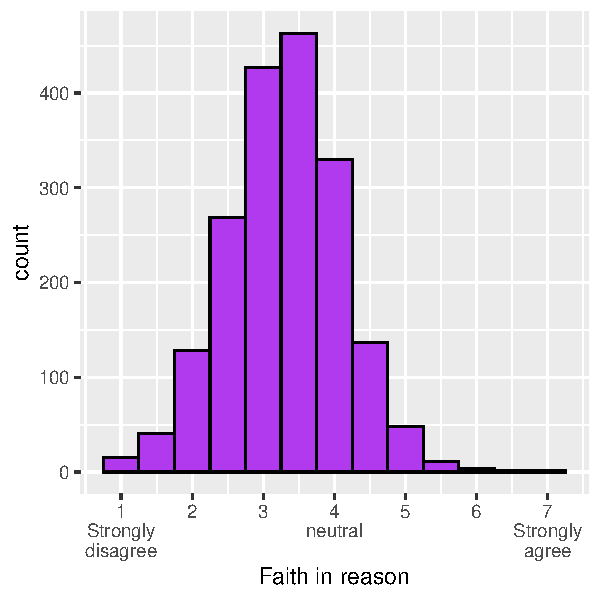
\includegraphics[width=0.75\linewidth]{faithinreason_files/figure-latex/meanhistogram-1} 

}

\caption{Histogram of mean of responses to all rationality items}\label{fig:meanhistogram}
\end{figure}

The average score across these six items was 3.29, a summary statistic which suggests that the typical view of other people weighted to being slightly less, rather than slightly more, reasonable. The distribution is shown in Figure \ref{fig:meanhistogram}.

\begin{figure}

{\centering 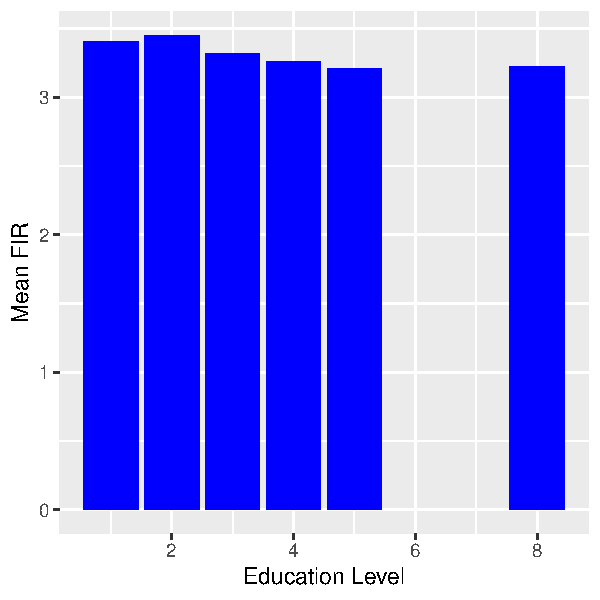
\includegraphics[width=0.75\linewidth]{faithinreason_files/figure-latex/education-1} 

}

\caption{Education level and mean FIR}\label{fig:education}
\end{figure}
\begin{figure}

{\centering 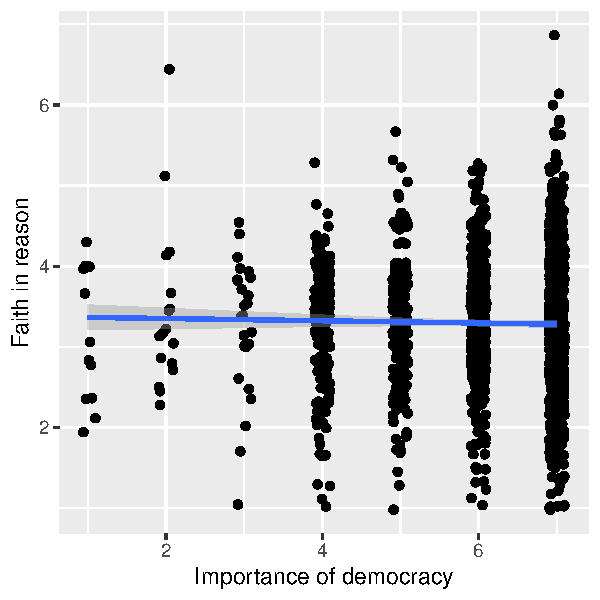
\includegraphics[width=0.75\linewidth]{faithinreason_files/figure-latex/democract-1} 

}

\caption{How important is it for you to live in a country that is governed democratically? and mean FIR. Note 0.1 jitter applied to x-axes values to allow visualisation of point density.}\label{fig:democract}
\end{figure}

\begin{figure}

{\centering 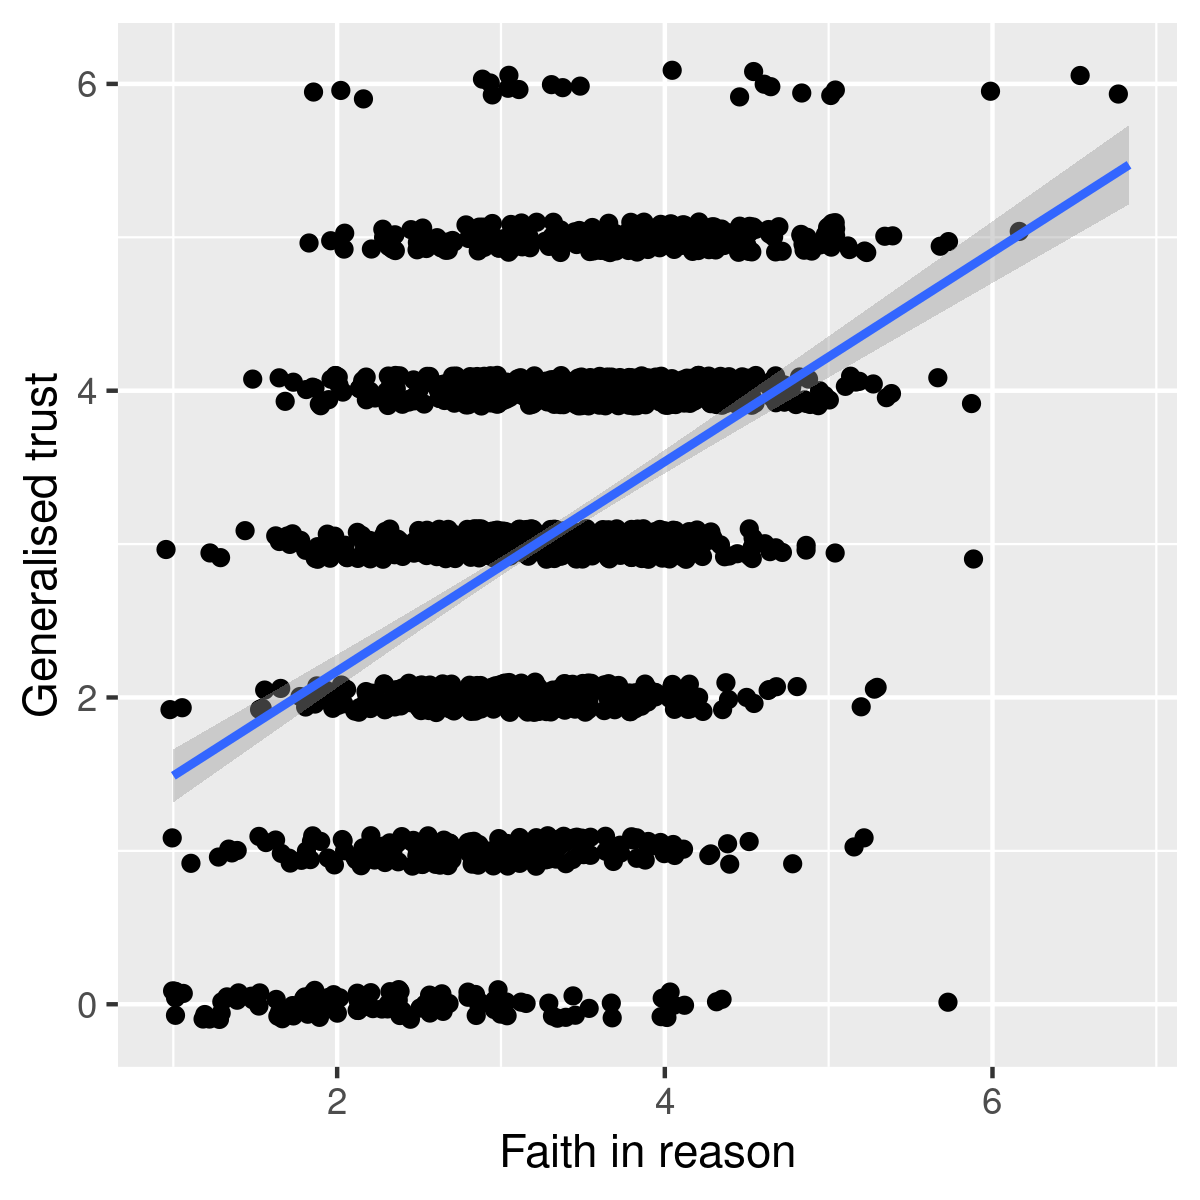
\includegraphics[width=0.75\linewidth]{faithinreason_files/figure-latex/generalisetrust-1} 

}

\caption{Generally speaking, would you say that most people can be trusted? and mean FIR. Note 0.1 jitter applied to x-axes values to allow visualisation of point density}\label{fig:generalisetrust}
\end{figure}

Relation to other variables
Regressions and corellations

\begin{figure}

{\centering 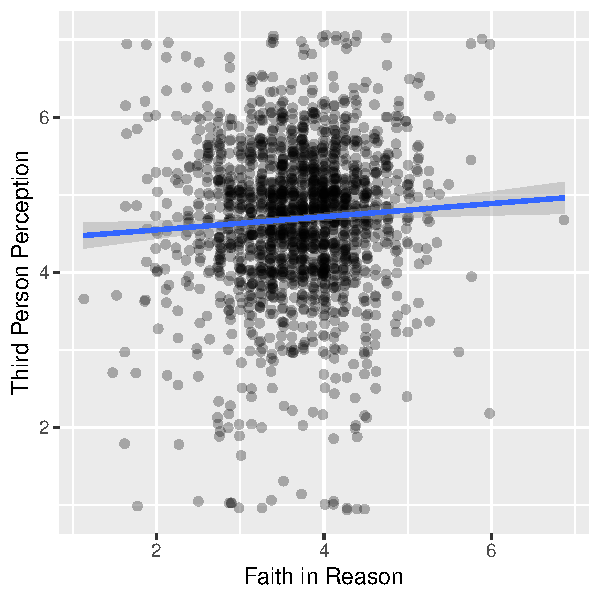
\includegraphics[width=0.75\linewidth]{faithinreason_files/figure-latex/tpe-1} 

}

\caption{Scatterplot of Faith in Reason scores against Third Person Effect score. Note 0.1 jitter applied to x-axes values to allow visualisation of point density}\label{fig:tpe}
\end{figure}

\hypertarget{todo}{%
\subsection{TODO}\label{todo}}

Analyse TPE

Methods for assessing dimensionality
cronbach's alpha + leave on out
scree plots and EFA
Mokken scale analysis
EGA

Write up all of them?

Look at items and make sensible decisions. A single scale of 6 items and 2 subscales?

\hypertarget{junyan}{%
\subsection{Junyan}\label{junyan}}

We asked 8 questions about rationality in the survey. To determine the homogeneity and the
fitness of the responses, I use Stata to perform Mokken scaling analysis. Testing all 8
rationality variables, the Mokken analysis yields one scale of 6 items. The items with low
Loevinger's coefficient of homogeneity (H i ), a criterion for scalability, are dropped. If the
overall H\textless0.3, it means the items in the scale are unrelated, thus cannot be accepted to form a
cumulative scale. As a rule of thumb, H i must be higher than 0.3 to be kept in the scale.
Therefore, there are 6 fitting items in the scale: rationality\_1, rationality\_2, rationality\_3,
rationality\_4, rationality\_6, and rationality\_7. The overall H coefficient is 0.41, indicating a
medium-strong scalability. The individual critical values in the scale are all lower than 80, so
the variables are double monotonous and there is no model violation.
Code: loevh rationality\_1 rationality\_2 rationality\_3 rationality\_4 rationality\_6 rationality\_7,
pair monotonicity(*) ppp pmm nipmatrix(minvi(0.03) siglevel(0.01))
We can thus generate a rationality variable by aggregating those six variables. Cronbach's \(\alpha\)
is 0.78, indicating an acceptable internal consistency.

Based on the statistical results, it looks to me that rationality\_5 (The average person can be
persuaded to change if given good reasons) is a real problem, it doesn't fit at all with other items

3
and must be removed. Rationality\_8 (People\textquotesingle s behaviour is generally consistent with their beliefs)
has a poor fitness, but it is not as bad as rationality\_5.

Next, I try to scale the remaining two items that are not included in the above scale --
rationality\_5 and rationality\_8. As expected, these two items doesn't form a separate scale.
Empirically, these items are excluded from the rationality measure by Mokken scaling likely
because persuasion effect is not a robust indication of rationality?

\hypertarget{tom}{%
\subsection{Tom}\label{tom}}

Obviously 5 is weakly correlated. Omitting gives biggest boost to Cronbach's alpha, EEGnet suggests weakly related to all other items,

EEGnet suggets two commuities
Scree plot of factors suggests border of unidimension and bidimensional
mokken analysis suggests 1 domension, BUT if you remove items 5 and 9 you then find 2 dim3nsions at 0.35

\hypertarget{discussion}{%
\section{Discussion}\label{discussion}}

This paper arose out of a note published online (Stafford, 2022) which we cite for completeness and by way of allowed it to be checked that the intention of the study has been consistent between conceptualisation and publication.

\hypertarget{scale-development}{%
\subsection{scale development}\label{scale-development}}

Usefully reviewed in Flake and Fried (2020); Clark and Watson (2019); Boateng, Neilands, Frongillo, Melgar-Quiñonez, and Young (2018)

We do not pretend to have completed scale development and testing, but aim to present the beginnings here.

\hypertarget{normative-models}{%
\subsection{Normative models}\label{normative-models}}

arguably our scale doesn't touch on normative models of rationality as captured by T\&K. Bias, prejudice

Deflationary accounts of misinformation (Mercier, 2020; Nyhan, 2020)

\hypertarget{references}{%
\section*{References}\label{references}}
\addcontentsline{toc}{section}{References}

\hypertarget{refs}{}
\begin{CSLReferences}{1}{0}
\leavevmode\vadjust pre{\hypertarget{ref-rmarkdowncite}{}}%
Allaire, J., Xie, Y., McPherson, J., Luraschi, J., Ushey, K., Atkins, A., \ldots{} Iannone, R. (2020). \emph{Rmarkdown: Dynamic documents for r}. Retrieved from \url{https://github.com/rstudio/rmarkdown}

\leavevmode\vadjust pre{\hypertarget{ref-altay2023}{}}%
Altay, S., \& Acerbi, A. (2023). People believe misinformation is a threat because they assume others are gullible. \emph{New Media \& Society}, 14614448231153379.

\leavevmode\vadjust pre{\hypertarget{ref-aust2020}{}}%
Aust, F., \& Barth, M. (2020). \emph{{papaja}: {Create} {APA} manuscripts with {R Markdown}}. Retrieved from \url{https://github.com/crsh/papaja}

\leavevmode\vadjust pre{\hypertarget{ref-boateng2018}{}}%
Boateng, G. O., Neilands, T. B., Frongillo, E. A., Melgar-Quiñonez, H. R., \& Young, S. L. (2018). Best practices for developing and validating scales for health, social, and behavioral research: A primer. \emph{Frontiers in Public Health}, \emph{6}, 149.

\leavevmode\vadjust pre{\hypertarget{ref-brand2022}{}}%
Brand, C. O., \& Stafford, T. (2022). Using dialogues to increase positive attitudes towards COVID-19 vaccines in a vaccine-hesitant UK population. \emph{Royal Society Open Science}, \emph{9}(10), 220366.

\leavevmode\vadjust pre{\hypertarget{ref-brehm1997}{}}%
Brehm, J., \& Rahn, W. (1997). Individual-level evidence for the causes and consequences of social capital. \emph{American Journal of Political Science}, 999--1023.

\leavevmode\vadjust pre{\hypertarget{ref-chung2016}{}}%
Chung, S., \& Moon, S.-I. (2016). Is the third-person effect real? A critical examination of rationales, testing methods, and previous findings of the third-person effect on censorship attitudes. \emph{Human Communication Research}, \emph{42}(2), 312--337.

\leavevmode\vadjust pre{\hypertarget{ref-clark2019}{}}%
Clark, L. A., \& Watson, D. (2019). Constructing validity: New developments in creating objective measuring instruments. \emph{Psychological Assessment}, \emph{31}(12), 1412.

\leavevmode\vadjust pre{\hypertarget{ref-cohn2019}{}}%
Cohn, A., Maréchal, M. A., Tannenbaum, D., \& Zünd, C. L. (2019). Civic honesty around the globe. \emph{Science}, \emph{365}(6448), 70--73.

\leavevmode\vadjust pre{\hypertarget{ref-davison1983}{}}%
Davison, W. P. (1983). The third-person effect in communication. \emph{Public Opinion Quarterly}, \emph{47}(1), 1--15.

\leavevmode\vadjust pre{\hypertarget{ref-dawson2009}{}}%
Dawson, N. V., \& Gregory, F. (2009). Correspondence and coherence in science: A brief historical perspective. \emph{Judgment and Decision Making}, \emph{4}(2), 126--133.

\leavevmode\vadjust pre{\hypertarget{ref-eiser2009}{}}%
Eiser, J. R., Stafford, T., Henneberry, J., \& Catney, P. (2009). {``Trust me, i'm a scientist (not a developer)''}: Perceived expertise and motives as predictors of trust in assessment of risk from contaminated land. \emph{Risk Analysis: An International Journal}, \emph{29}(2), 288--297.

\leavevmode\vadjust pre{\hypertarget{ref-feng2012}{}}%
Feng, G. C., \& Guo, S. Z. (2012). Support for censorship: A multilevel meta-analysis of the third-person effect. \emph{Communication Reports}, \emph{25}(1), 40--50.

\leavevmode\vadjust pre{\hypertarget{ref-flake2020}{}}%
Flake, J. K., \& Fried, E. I. (2020). Measurement schmeasurement: Questionable measurement practices and how to avoid them. \emph{Advances in Methods and Practices in Psychological Science}, \emph{3}(4), 456--465.

\leavevmode\vadjust pre{\hypertarget{ref-furnham1985}{}}%
Furnham, A., Johnson, C., \& Rawles, R. (1985). The determinants of beliefs in human nature. \emph{Personality and Individual Differences}, \emph{6}(6), 675--684.

\leavevmode\vadjust pre{\hypertarget{ref-gss}{}}%
General Social Survey Team. (2023). \emph{General social survey}. Available at: \url{https://gss.norc.org}.

\leavevmode\vadjust pre{\hypertarget{ref-gigerenzer2011}{}}%
Gigerenzer, G., \& Gaissmaier, W. (2011). Heuristic decision making. \emph{Annual Review of Psychology}, \emph{62}, 451--482.

\leavevmode\vadjust pre{\hypertarget{ref-hoes2022}{}}%
Hoes, E., Clemm von Hohenberg, B., Gessler, T., Wojcieszak, M., \& Qian, S. (2022). \emph{The cure worse than the disease? How the media's attention to misinformation decreases trust}. PsyArXiv. \url{https://doi.org/10.31234/osf.io/4m92p}

\leavevmode\vadjust pre{\hypertarget{ref-holcombe2020documenting}{}}%
Holcombe, A. O., Kovacs, M., Aust, F., \& Aczel, B. (2020). Documenting contributions to scholarly articles using CRediT and tenzing. \emph{PLoS One}, \emph{15}(12), e0244611.

\leavevmode\vadjust pre{\hypertarget{ref-wvs}{}}%
Inglehart, C., R., \& Team, W. (2023). \emph{World values survey}. Available at: \url{https://www.worldvaluessurvey.org}.

\leavevmode\vadjust pre{\hypertarget{ref-jungherr2022}{}}%
Jungherr, A., \& Rauchfleisch, A. (2022). \emph{Negative downstream effects of disinformation discourse: Evidence from the US}. SocArXiv.

\leavevmode\vadjust pre{\hypertarget{ref-kahneman1982}{}}%
Kahneman, D., Slovic, S. P., \& Tversky, A. (1982). \emph{Judgment under uncertainty: Heuristics and biases}. Cambridge university press.

\leavevmode\vadjust pre{\hypertarget{ref-karadzhov2022}{}}%
Karadzhov, G., Stafford, T., \& Vlachos, A. (2022). What makes you change your mind? An empirical investigation in online group decision-making conversations. \emph{arXiv Preprint arXiv:2207.12035}.

\leavevmode\vadjust pre{\hypertarget{ref-karpf2019}{}}%
Karpf, D. (2019). On digital disinformation and democratic myths. Retrieved from \url{https://mediawell.ssrc.org/expert-reflections/on-digital-disinformation-and-democratic-myths/}

\leavevmode\vadjust pre{\hypertarget{ref-lee2021}{}}%
Lee, T. (2021). How people perceive influence of fake news and why it matters. \emph{Communication Quarterly}, \emph{69}(4), 431--453.

\leavevmode\vadjust pre{\hypertarget{ref-lyons2022}{}}%
Lyons, B. A. (2022). Why we should rethink the third-person effect: Disentangling bias and earned confidence using behavioral data. \emph{Journal of Communication}, \emph{72}(5), 565--577.

\leavevmode\vadjust pre{\hypertarget{ref-mercier2020}{}}%
Mercier, H. (2020). \emph{Not born yesterday}. Princeton: Princeton University Press.

\leavevmode\vadjust pre{\hypertarget{ref-mercier2011}{}}%
Mercier, H., \& Sperber, D. (2011). Why do humans reason? Arguments for an argumentative theory. \emph{Behavioral and Brain Sciences}, \emph{34}(2), 57--74.

\leavevmode\vadjust pre{\hypertarget{ref-nisbet2021}{}}%
Nisbet, E. C., Mortenson, C., \& Li, Q. (2021). The presumed influence of election misinformation on others reduces our own satisfaction with democracy. \emph{Harvard Kennedy School Misinformation Review}.

\leavevmode\vadjust pre{\hypertarget{ref-nisbett1977}{}}%
Nisbett, R. E., \& Wilson, T. D. (1977). Telling more than we can know: Verbal reports on mental processes. \emph{Psychological Review}, \emph{84}(3), 231.

\leavevmode\vadjust pre{\hypertarget{ref-nyhan2020facts}{}}%
Nyhan, B. (2020). Facts and myths about misperceptions. \emph{Journal of Economic Perspectives}, \emph{34}(3), 220--236.

\leavevmode\vadjust pre{\hypertarget{ref-olshansky2020}{}}%
Olshansky, A., \& Landrum, A. R. (2020). Third-person perceptions and calls for censorship of flat earth videos on YouTube. \emph{Media and Communication}, \emph{8}(2), 387--400.

\leavevmode\vadjust pre{\hypertarget{ref-pascal1910}{}}%
Pascal, B. (1669/1910). \emph{Thoughts} (Vol. 48). PF Collier \& son. Retrieved from \url{\%22http://entersection.com/posts/1189-blaise-pascal-on-man-as-a-thinking-reed\%22}

\leavevmode\vadjust pre{\hypertarget{ref-paxton1999}{}}%
Paxton, P. (1999). Is social capital declining in the united states? A multiple indicator assessment. \emph{American Journal of Sociology}, \emph{105}(1), 88--127.

\leavevmode\vadjust pre{\hypertarget{ref-perloff2002}{}}%
Perloff, R. M. (2002). The third-person effect. In \emph{Media effects} (pp. 499--516). Routledge.

\leavevmode\vadjust pre{\hypertarget{ref-putnam2000}{}}%
Putnam, R. D. (2000). \emph{Bowling alone: The collapse and revival of american community}. Simon; schuster.

\leavevmode\vadjust pre{\hypertarget{ref-samuels2002}{}}%
Samuels, R., Stich, S., \& Bishop, M. (2002). {236Ending the Rationality Wars How to Make Disputes about Human Rationality Disappear}. In \emph{{Common Sense, Reasoning, and Rationality}}. Oxford University Press. \url{https://doi.org/10.1093/0195147669.003.0011}

\leavevmode\vadjust pre{\hypertarget{ref-sommer2022}{}}%
Sommer, J., Musolino, J., \& Hemmer, P. (2022). A hobgoblin of large minds: Troubles with consistency in belief. \emph{Wiley Interdisciplinary Reviews: Cognitive Science}, e1639.

\leavevmode\vadjust pre{\hypertarget{ref-stafford2014}{}}%
Stafford, T. (2014). The perspectival shift: How experiments on unconscious processing don't justify the claims made for them. \emph{Frontiers in Psychology}, \emph{5}, 1067. \url{https://doi.org/10.3389/fpsyg.2014.01067}

\leavevmode\vadjust pre{\hypertarget{ref-stafford2020evidence}{}}%
Stafford, T. (2020). Evidence for the rationalisation phenomenon is exaggerated. \emph{Behavioral and Brain Sciences}, \emph{43}.

\leavevmode\vadjust pre{\hypertarget{ref-stafford2022}{}}%
Stafford, T. (2022, May 8). Quantifying our faith in reason. Retrieved from \url{https://tomstafford.substack.com/p/quantifying-our-faith-in-reason}

\leavevmode\vadjust pre{\hypertarget{ref-stavrova2016}{}}%
Stavrova, O., \& Ehlebracht, D. (2016). Cynical beliefs about human nature and income: Longitudinal and cross-cultural analyses. \emph{Journal of Personality and Social Psychology}, \emph{110}(1), 116.

\leavevmode\vadjust pre{\hypertarget{ref-stojanov2020}{}}%
Stojanov, A., Bering, J. M., \& Halberstadt, J. (2020). Does perceived lack of control lead to conspiracy theory beliefs? Findings from an online MTurk sample. \emph{PLoS One}, \emph{15}(8), e0237771.

\leavevmode\vadjust pre{\hypertarget{ref-stojanov2019}{}}%
Stojanov, A., \& Halberstadt, J. (2019). The conspiracy mentality scale. \emph{Social Psychology}, \emph{50}, 215-\/-232. \url{https://doi.org/10.1027/1864-9335/a000381}

\leavevmode\vadjust pre{\hypertarget{ref-sun2008}{}}%
Sun, Y., Pan, Z., \& Shen, L. (2008). Understanding the third-person perception: Evidence from a meta-analysis. \emph{Journal of Communication}, \emph{58}(2), 280--300.

\leavevmode\vadjust pre{\hypertarget{ref-swami2017}{}}%
Swami, V., Barron, D., Weis, L., Voracek, M., Stieger, S., \& Furnham, A. (2017). An examination of the factorial and convergent validity of four measures of conspiracist ideation, with recommendations for researchers. \emph{PloS One}, \emph{12}(2), e0172617.

\leavevmode\vadjust pre{\hypertarget{ref-zhu2023}{}}%
Zhu, J., Dommett, K., \& Stafford, T. (submitted). \emph{What makes online political ads unacceptable? Interrogating public attitudes to inform regulatory responses}.

\end{CSLReferences}


\end{document}
